\documentclass[11pt]{article}

\usepackage[margin=1in]{geometry}

\usepackage{mathpazo}
\usepackage{graphicx}
%\usepackage{cite}

\newcommand{\gcc}{\mathrm{g~cm^{-3} }}
\newcommand{\castro}{{\sffamily{Castro}}}

\begin{document}

\begin{center}
  {\Large Notes on the Black Widow Pulsar Problem}
\end{center}

\section{\castro\ Setup}
The setup consists of a $0.2 M_\odot$ star receiving gray radiation to the right. 

\subsection{Star's initial model}
For the initial model I used the code in MAESTRO/Util/initial\_models/spherical. We are working under the assumption that at this point the star is fully convective and therefore isentropic.\\

To start the study we will be using {\tt EOS\_dir = gamma\_law\_general } for the equation of state. The star has sun like composition so I'm using {\tt network\_inputs = H\_He.net}. For this assumptions we can use a Polytrope
\begin{equation}
	P(r) = K \rho^{1+\frac{1}{n}}(r)
\end{equation}

with $n=3/2$ since it is fully convective and ideal gas. To estimate some of the parameters for the inputs for this code, I'm using the fact that I want $0.2 M_\odot$ mass and some central temperature of around $10^7 K$. With that in mind we can get the radius using \cite{hansen2004stellar}:
\begin{equation}
	T_c = \frac{2.293 \times 10^7}{(n+1)(-\xi \theta'_n)_{\xi _1}} \mu \left(\frac{M}{M_\odot}\right)\left(\frac{R}{R_\odot}\right)^{-1} 
\end{equation}

The tabulated values for $\xi_1 = 3.65375$ and $-\xi_1^2 \left(\frac{d\theta}{d\xi}\right)_{\xi _1} = 2.71406$ giving $\frac{R}{R_\odot} \simeq 0.15$. Now, we can obtain $P_c$ with :

\begin{equation}
	P_c = \frac{8.952 \times 10^{14}}{(n+1)(\theta'_n)^2_{\xi _1}} \left(\frac{M}{M_\odot}\right)\left(\frac{R}{R_\odot}\right)^{-4}
\end{equation}

Resulting with $P_c \simeq 6.845 \times 10^{17} \quad dyne \quad cm^{-2}$. Using the ideal gas law: 
\begin{equation}
	P_c = \frac{\rho_c N_A k T_c}{\mu}
\end{equation}
Which gives us a central density of $\rho_c \simeq 493$.\\

With that information the input parameters that I ended up using were:
\begin{itemize}

	\item {\tt nx = 1280}
	\item {\tt dens\_base = 4.97d2}
	\item {\tt temp\_base = 2.02e7}
	\item {\tt temp\_fluff = 4.1e3}
	\item {\tt low\_density\_cutoff = 1.4d-6}
	\item {\tt M\_conv\_zone = 1.5d1}
	\item {\tt xmin = 0.0}
	\item {\tt xmax = 1.2e10}
	\item {\tt cfrac = 0.75}

\end{itemize}

The final star properties are:
\begin{itemize}
	\item $M = 0.1995 M_\odot$
	\item $R \sim 1.04 \times 10^{10}$
	\item surface Temperature $T = 4151.15$
	\item surface density $\rho = 1.46 \times 10^{-3}$
\end{itemize}

\subsubsection{Code changes}
The changes I did in the {\tt init\_1d.f90} code were: 
\begin{enumerate}
	\item comment lines that contain {\tt use\_eos\_coulomb} which is necessary for helmholtz eos but not used for gamma law.
	
	\item composition indices from network module 
	\item Added an if at the last print so that if it is isentropic at the end (which should be in our case) the print of convective mass will show the same as the total mass.  
\end{enumerate}


\subsection{Some yt plots}

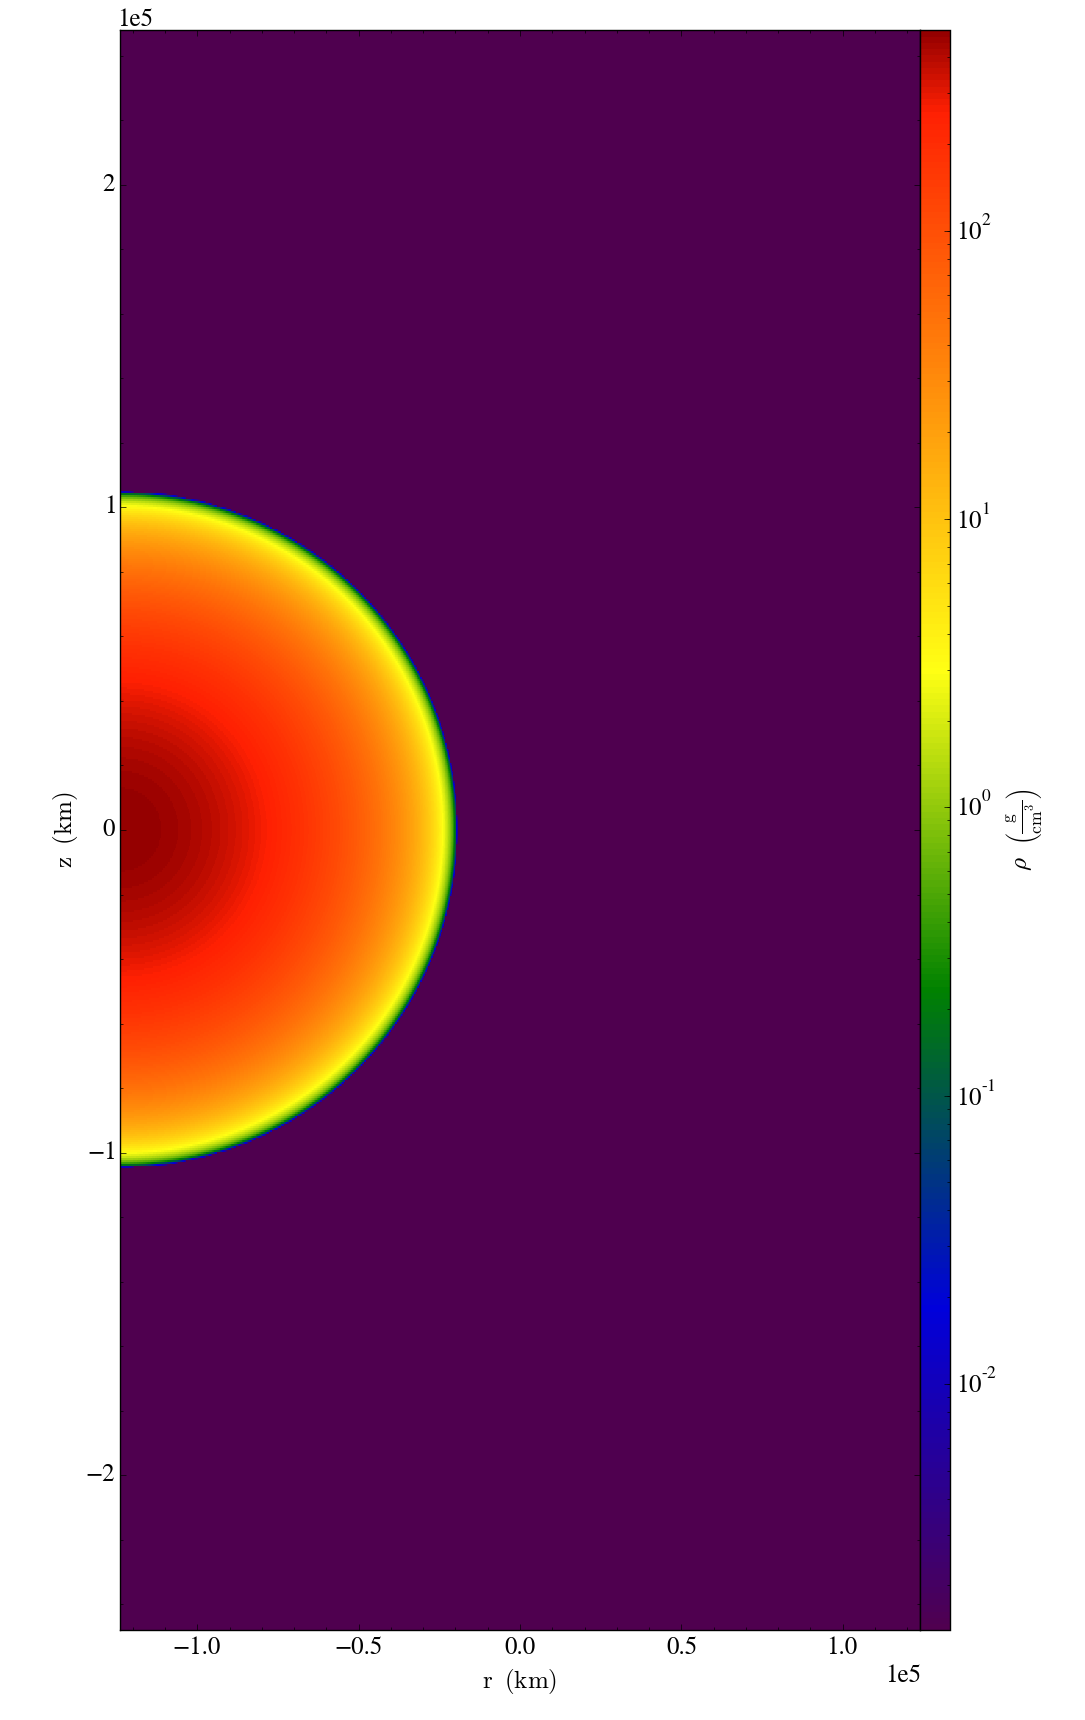
\includegraphics[width=0.60\textwidth]{_Slice_theta_density.png}

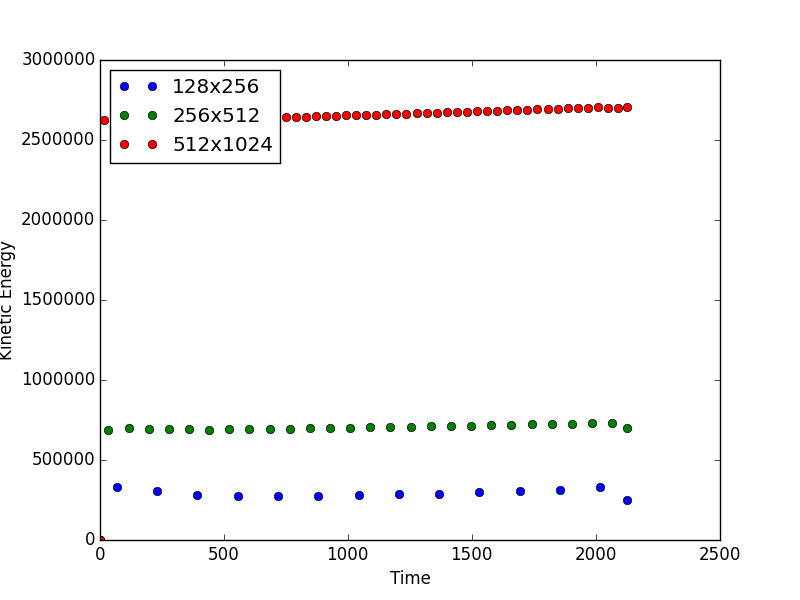
\includegraphics[width=0.65\textwidth]{KEvsT.png}

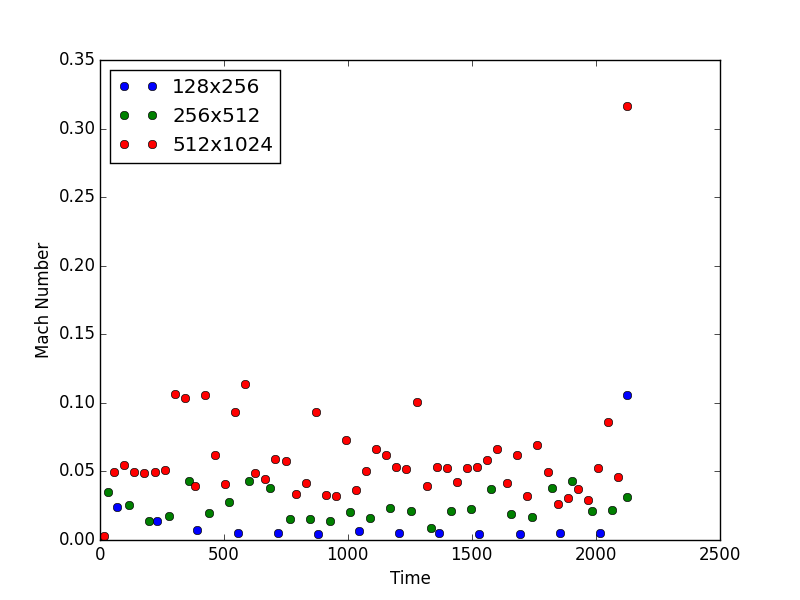
\includegraphics[width=0.65\textwidth]{mNumber.png}

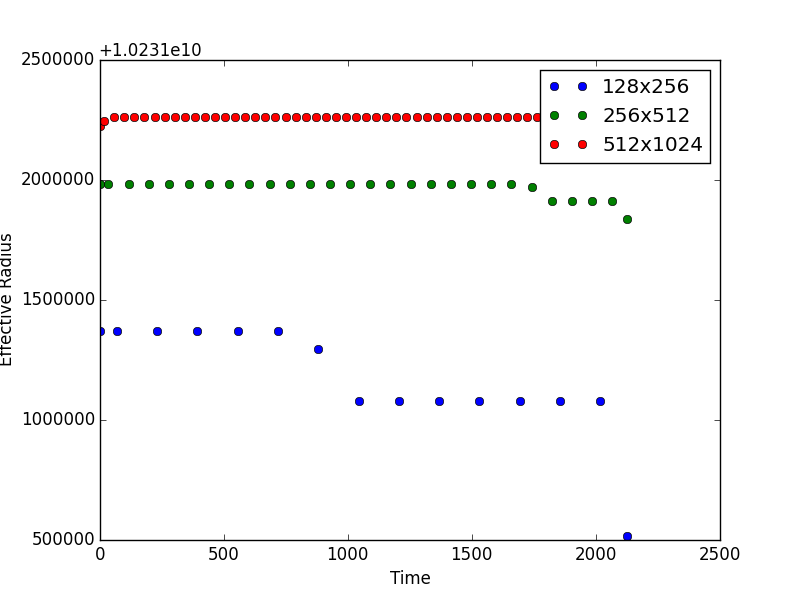
\includegraphics[width=0.65\textwidth]{ReffvsT.png}

\section{\castro\ Radiation Solver Details}

We are using the gray radiation solver.  
\begin{itemize}
\item {\tt radiation.comoving = 0} 
\item {\tt radsolve.level\_solver\_flag = 104} 
\item {\tt castro.cfl}: the value I'm using is {\tt
  0.8}
\end{itemize}


\section{Opacity}

We are using Kramers opacity law \cite{carroll2007introduction}:
\begin{equation}
  \tilde{\kappa} = \tilde{\kappa}_0 \frac{\rho}{T^{3.5}} 
\end{equation}

The approximation formulae developed for average bound-free and free-free opacities go like \cite{hansen2004stellar}:

\begin{equation}
  \tilde{\kappa}_{bf} = 4 \times 10^{25} Z(1+X) \frac{\rho}{T^{3.5}} ~\mathrm{cm^{2}g^{-1}}
\end{equation}

\begin{equation}
  \tilde{\kappa}_{ff} = 4 \times 10^{22} (X+Y)(1+X) \frac{\rho}{T^{3.5}} ~\mathrm{cm^{2}g^{-1}}
\end{equation}

Where $X$, $Y$ and $Z$ are the hydrogen, helium and metal mass fractions. 

Note that this form of opacity has different units than what \castro\ uses.  For \castro\,
opacity has units of $\mathrm{cm^{-1}}$, so we have:
\begin{equation}
  \kappa = \rho \tilde{\kappa} = \tilde{\kappa}_0 \frac{\rho^2}{T^{3.5}}
\end{equation}
 

\castro\ takes the opacity as a simple power law of density and temperature (without any reference values for scaling).

Since \castro\ wants $\kappa = \kappa_0 \rho^m T^{-n}$, we evaluate this with $\rho = 1~\gcc$ and $T = 1~\mathrm{K}$:
\begin{equation}
  \kappa = 3.8 \times 10^{22} \, \rho^2 T^{-3.5}~\mathrm{cm^{-1}}
\end{equation}
This can be set in \castro\ as:
\begin{verbatim}
radiation.const_kappa_p = 3.8e22
radiation.kappa_p.exp_m = 2
radiation.kappa_p_exp_n = 3.5
\end{verbatim}


\subsection{Boundary Conditions}

The z boundary of the domain specifies the flux coming from
the pulsar.  For the planet problem Weiqun suggested the Sanchez-Pomraning BC, which is a Neumann-like BC that allows for an incoming and outgoing flux.

The planet notes give the following explanation which I modified for this problem. The form of the flux is $F = cE_r$, where $E_r$ is the radiation energy density.  This flux has units of $\mathrm{erg~cm^{-2}~s^{-1}}$.
We can obtain the flux using:
\begin{equation}
  f = \frac{L_\star}{4\pi d^2}
\end{equation}
where $L_\star$ is the luminosity of the pulsar and $d$ is the
distance between the companion and the pulsar.


   From \cite{0004-637X-769-2-108}, using values for B1952+20,  $L_\star = 2\times 10^{33}\mathrm{erg~s^{-1}}$ and $d = 2.49R_\odot$,  we get $f =
5.3\times 10^9~\mathrm{erg~cm^{-2}~s^{-1}}$.

Since at the moment we were not seeing the flux, now we are using $5\times 10^15$ 

   \subsection{bc\_fill\_2d.f90}
   We will be modifying the subroutine ca\_radfill so that the hyperbolic BC for the radiation energy take into account the radiation flux entering the boundary? For that we can take a similar approach than the mention in \cite{advinrad} using 
   
   $$F_{in} = \frac{c}{4} E_r - \frac{1}{2}$$
   $$F_{out} = \frac{c}{4} E_r + \frac{1}{2}$$
   


%\nocite{*}
\bibliography{references}{}
\bibliographystyle{plain}

\end{document}
